\chapter{Optimizing the Execution of Large Scale Scientific Workflows in Public Clouds}
\label{chapter:dewe_v1}

\section{Introduction}
\label{sec:dewe_v1:dewe_v1_intro}

In recent years, the concept of workflow has gained increasing level of acceptance by the scientific computing community. Large-scale scientific computations usually involve a large number of different tasks, often in the number of hundreds or thousands. Some of these tasks depend on the output of other tasks (i.e., precedence constraints), forming a workflow. When the precedence requirements for certain tasks have been met, each of these tasks can then run independently in its own environment. In practice, scientific workflows are usually run on clusters with multiple computing nodes. A workflow management system is needed to control the sequence of task execution, computing resource assignment, as well as data transfer to satisfy the precedence constraints. 

Examples of scientific workflows are Montage \cite{montage, web:montage}, LIGO \cite{ligo}, and CyberShake \cite{cybershake}. Examples of workflow management systems are Pegasus \cite{deelman2004pegasus} and Kepler \cite{altintas2004kepler}.

For many scientific workflow applications, the task modules are often developed as sequential code. One reason is that these modules were developed in early years when the concept of parallel programming had not been widely adopted by researchers in specific problem domains. Even today the development of parallel code is pretty complex for non experts in parallel programming. The other reason is that workflow management systems usually use CPU slots (e.g., cores, or virtual CPU cores or vCPUs) as basic resource allocation units, and it is easier to carry out workflow scheduling with a one-to-one mapping between CPU slots and tasks. Due to the precedence constraints between tasks, only certain tasks are eligible to run at a given point in time. When the number of concurrently running tasks is smaller than the number of CPU slots available in the computing cluster, the extra CPU slots will be idling. In the extreme case, only one task is running on one CPU slot in a large computing cluster, resulting in significant under-utilization of computing resources.

A workflow can be represented by a directed acyclic graph (DAG), where the vertices represent the tasks and the edges represent the precedence constraints. The DAG scheduling problem is NP-complete in general. In recent years, there emerged a large volume of literature on workflow scheduling, with the goal to decrease the time needed by the workflow or minimize the size/cost of the computing cluster. Other attempts to optimize workflow execution include using alternative data storage and data staging options for improved I/O efficiency. However, none of the existing methods addresses the resource under-utilization problem caused by sequential code, especially when certain sequential code becomes the bottleneck of a workflow. 

In this chapter, we present a set of methods to optimize the execution of scientific workflows, with the Montage astronomical mosaic engine running on Amazon EC2 as an example. We use our own DEWE (Distributed Elastic Workflow Execution)\footnote{DEWE including its source code and visualization toolkit used in this study is available from \url{https://bitbucket.org/lleslie/dwf/wiki/Home}.} as a workflow management system. The main contributions of the present work are:

\begin{itemize}
	\item We develop a workflow visualization toolkit to visualize the workflow execution process and resource consumption pattern. We use the workflow visualization toolkit to process the trace files produced by the workflow management system to identify the bottleneck of the Montage workflow.
	\item We compare the impact of compiler optimization on the performance of the Montage workflow, using both GNU C Compiler (GCC) and Intel C Compiler (ICC).  	
	\item We use parallelization techniques to optimize the mBgModel module in the Montage workflow, resulting in significant degree of performance gains.
	\item We compare the impact of different computing cluster configurations on Amazon EC2 on the performance of the Montage workflow, and analyze the root cause for the performance difference. 
\end{itemize}

The rest of this chapter is organized as follows. Section \ref{v1_sec:montage} provides an overview of the Montage workflow. Section \ref{v1_sec:visualization} describes the design of the workflow visualization toolkit and its usage. In Section \ref{v1_sec:parallel}, we discuss various optimization techniques for the Montage workflow, including compiler optimization (using different compiler with different optimization flags), parallelization of key jobs (parallelizing the mBgModel job in the workflow), as well as cluster configurations (using clusters with different EC2 instance types, but keep the hourly cost constant). We summarize our conclusions in Section \ref{v1_sec:summary}.

\section{The Montage Workflow}
\label{v1_sec:montage}


\begin{figure}[!t]
	\centering
	\hspace{-10pt}
	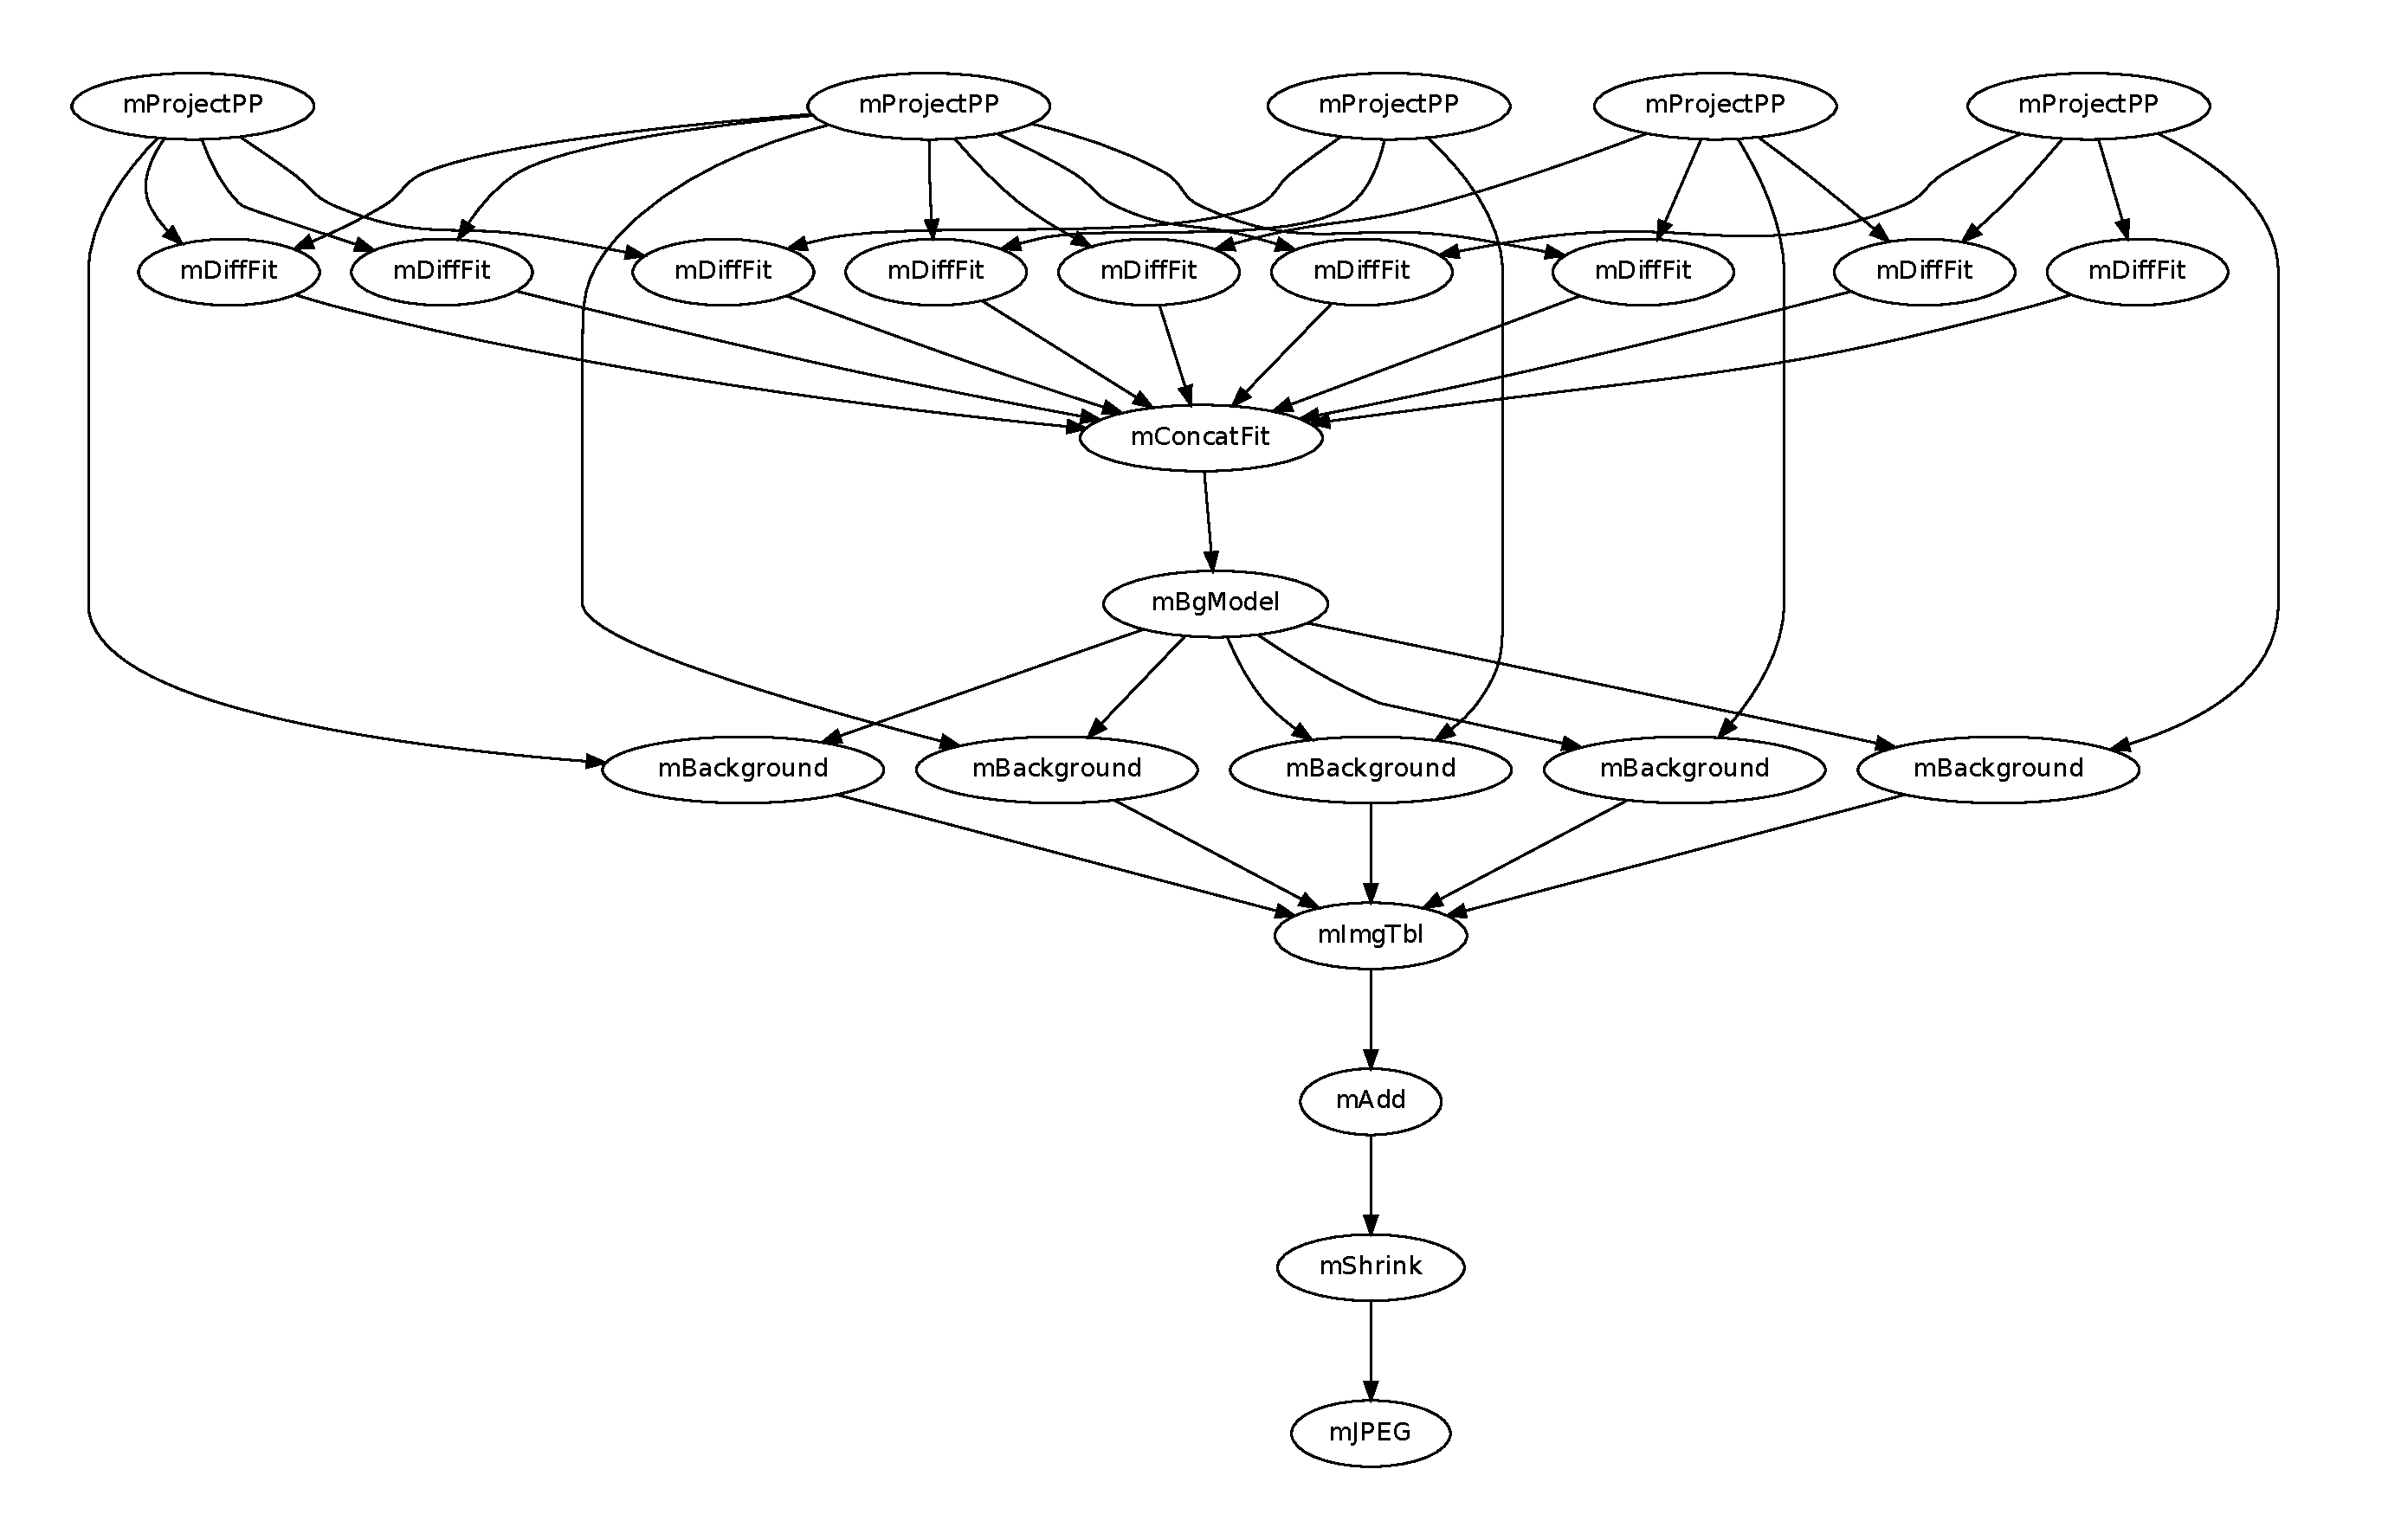
\includegraphics[width=9.7cm, height=7cm]{montage}
    \caption{The structure of the Montage workflow.}
    \vspace{-10pt}
	\label{v1_fig:montage}
\end{figure}


In this chapter, we choose Montage as a representative example of large scale scientific workflows for our case study. Montage is an astronomical image mosaic engine that assembles individual images of the sky into a mosaic. A 6.0 degree Montage workflow creates a 6-by-6 degree square mosaic centered at a particular region of the sky (e.g., M16). The number of jobs and input data files increases with the number of degrees of the mosaic. 

Figure \ref{v1_fig:montage} describes the structure of the Montage workflow. The progress of the workflow has a three-stage pattern. During the first stage, a large number of mProjectPP jobs run in parallel, followed by a large number of mDiffFit jobs running in parallel. During the second stage, two jobs mConcatFit and mBgModel run one after another, during which no other jobs are eligible to run. In this paper, we consider mConcatFit and mBgModel as blocking jobs because they block the execution of other jobs. During the third stage, a large number of mBackground jobs run in parallel, followed by a small number of mImgTbl, mAdd, mShrink, and mJPEG jobs.

A 6.0 degree Montage workflow contains 8,586 jobs, 1,444 input files with a total size of 4.0 GB, and 22,850 intermediate files with a total size of 35 GB. In practice, a set of smaller image mosaics are needed to produce a large image mosaic, where each smaller image mosaic is generated by a Montage workflow. For example, the Galaetic Plane workflow ensemble \cite{deelman2013hosted} consists of 17 workflows, each of which further contains 900 sub-workflows. In this chapter, we are more concern about the execution of a single Montage workflow in a public cloud environment. In the next chapter, we will discuss the execution of large-scale Montage workflow ensembles in public clouds.


\section{Workflow Visualization Toolkit}
\label{v1_sec:visualization}

\begin{figure}[t!]
\centering
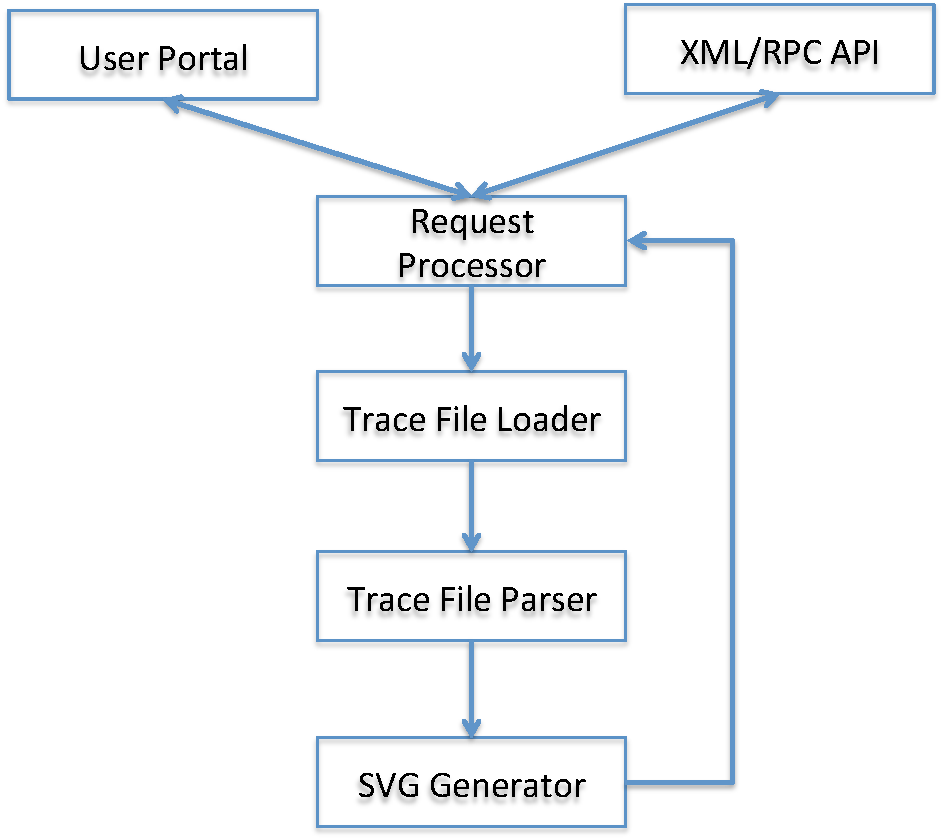
\includegraphics[width=8cm]{toolkit}
\caption{Design of Workflow Visualization Toolkit}
	\label{fig:toolkit}
\end{figure}



In this section, we present a workflow visualization toolkit that visualizes the workflow execution process and its resource consumption pattern. Figure \ref{fig:toolkit} shows the design of the workflow visualization toolkit. The user portal accepts user requests from a web browser, while the XML/RPC API accepts user requests from third party applications (such as workflow execution frameworks) via API calls. Both requests specify the type of visualization to produce, the format of the workflow trace file, the location of the workflow trace file in the form of a public accessible URL, along with some other parameters. The request handler receives these requests, and coordinates the different steps needed to produce the output vector graph. The trace file loader loads the workflow trace file from the URL specified by the user. The trace file parser extracts workflow execution information from the trace file and saves it into a data structure, as well as calculating the overall resource utilization rates for each worker node and CPU. The SVG generator produces the scalable vector graph (SVG) based on the parsed information saved in the data structure, and returns it to the request handler. The request handler then returns the output scalable vector graph to the user's browser or the third party application for further integration.

\begin{figure*}[ht]
\centering
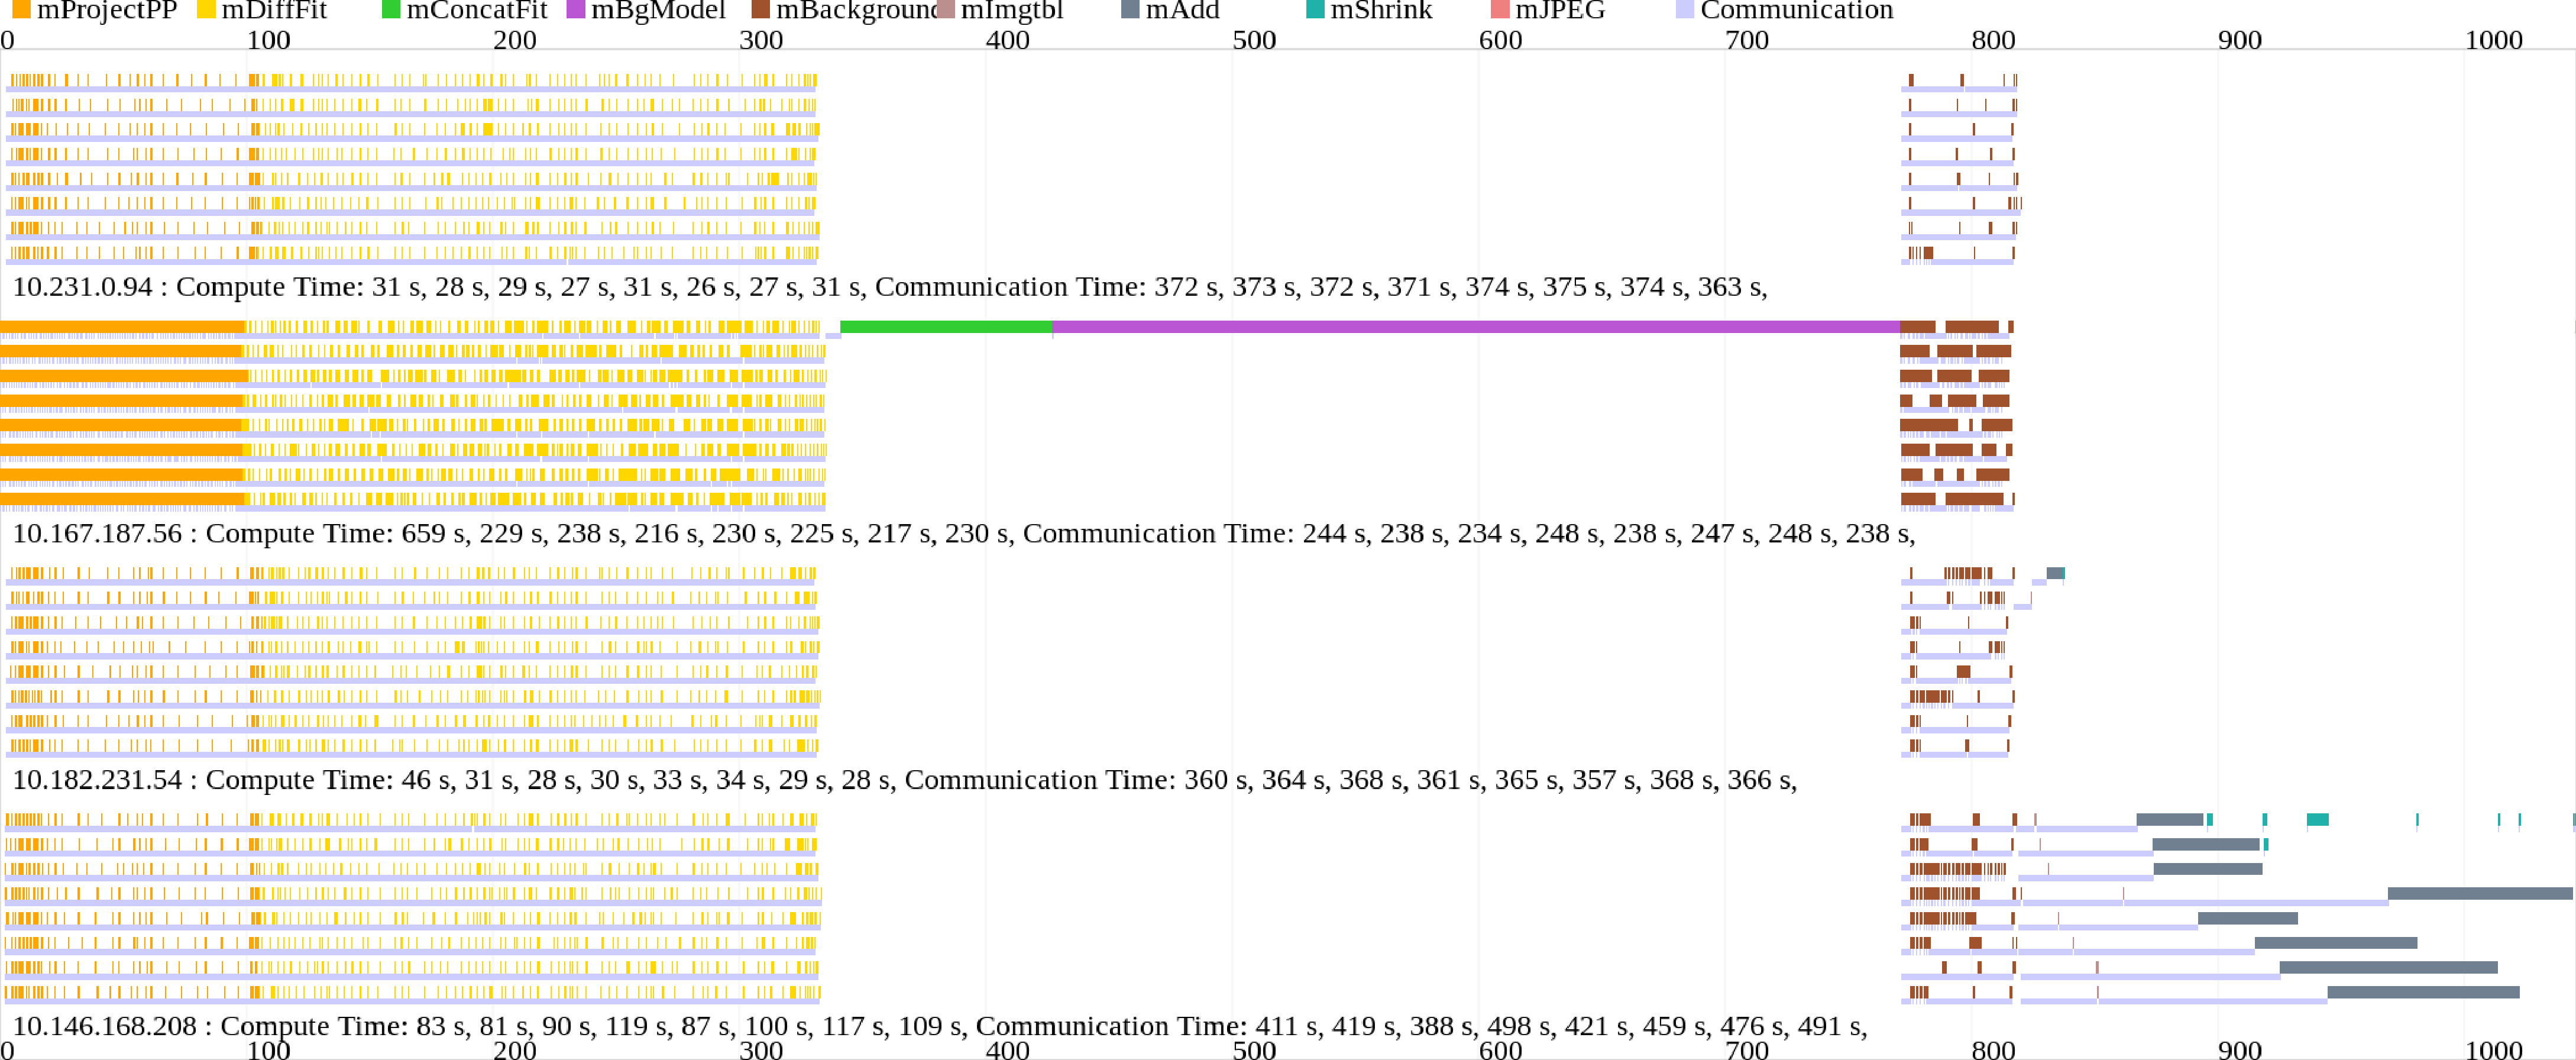
\includegraphics[width=16cm]{visual}
\caption{Detailed visualization of a 6.0 degree Montage workflow running Amazon EC2. The computing cluster includes 4 m3.2xlarge instances.}
\label{fig:detail}
\end{figure*}

\begin{figure*}[ht]
\centering
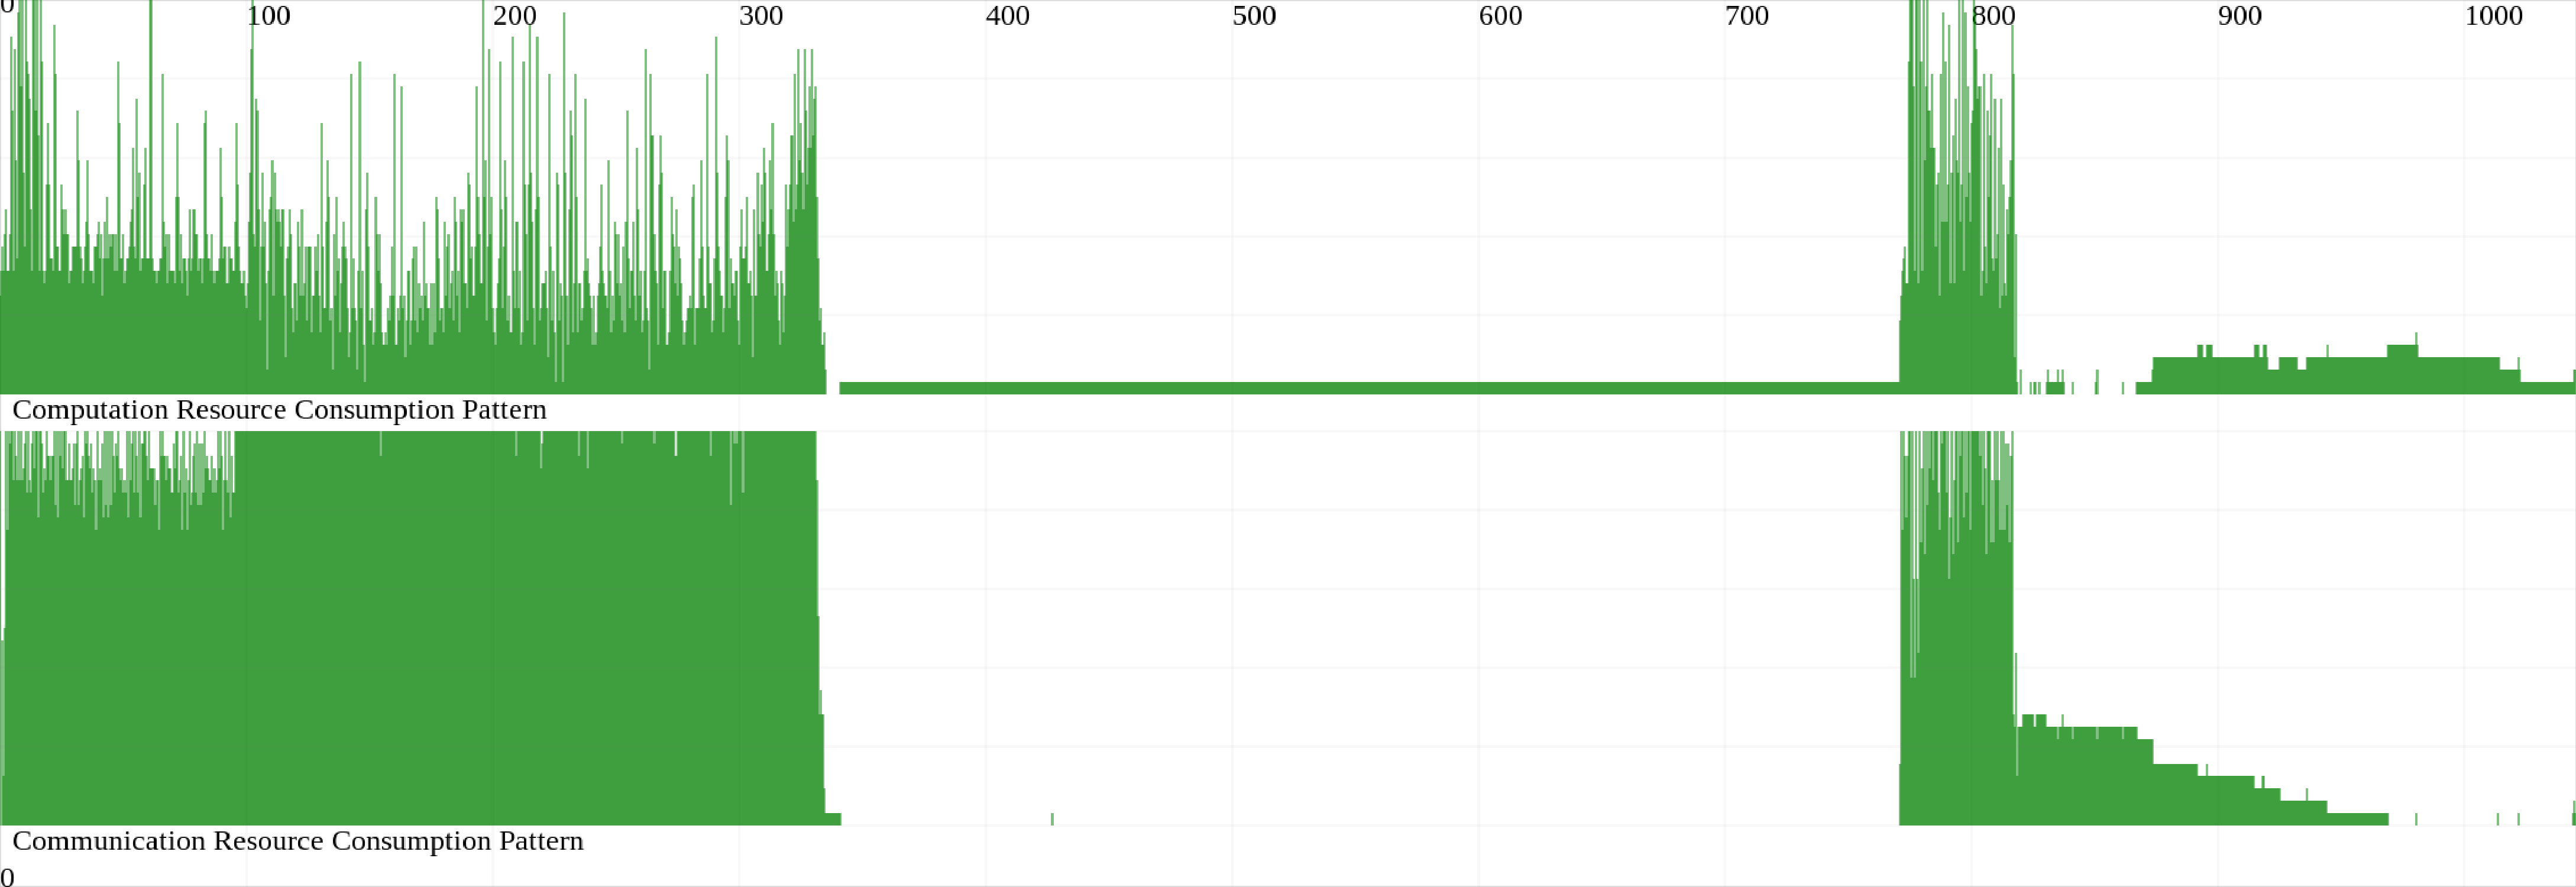
\includegraphics[width=16cm]{pattern}
\caption{Resource consumption pattern of a 6.0 degree Montage workflow running Amazon EC2. The computing cluster includes 4 m3.2xlarge instances.}
\label{fig:pattern}
\end{figure*}



The workflow visualization toolkit takes a workflow execution trace file as the input, and produces a scalable vector graph (SVG) representing the resource consumption status during the whole makespan. In a workflow execution detailed visualization, the scalable vector graph includes information about (a) each individual task with task coloring, such as task id, name of the binary, start time, task execution time, data transfer start time and data transfer execution time; and (b) summarized resource consumption information about each worker node and CPU in terms of computation time, communication time, and resource utilization rate. In a resource consumption pattern visualization (Figure \ref{fig:pattern}), the scalable vector graph provides resource consumption rate for both computation and communication resources, as defined by the ratio between the number of concurrently running computation or communication tasks and the number of total CPUs in the computing cluster.

The detailed visualization and  resource consumption patterns of a 6.0 degree Montage workflow running on Amazon EC2 are shown in Figures \ref{fig:detail} and \ref{fig:pattern}, respectively. The experiments are carried out on a cluster with 4 EC2 instances in the us-east-1 region. The instance type being used in the experiments is m3.2xlarge \footnote{The M3 product family is the current generation general purpose product family backed by Intel Xeon E5-2670 v2 (Sandy Bridge) processors and SSD storages. The m3.2xlarge instance is the biggest instance type in the M3 product family. Each m3.2xlarge instance has 8 vCPUs, 30 GB memory, and two 80 GB SSD ephemeral storages.} . Specifically, the computing cluster includes 4 m3.2xlarge instances, each of which has 8 vCPUs and 30 GB memory. The binaries are compiled with GCC with the -O2 compiler optimization flag. The makespan of the workflow is 1046 seconds, and the runtime of task mBgModel is 344 seconds. 


As shown in Figure  \ref{fig:detail}, and Figure \ref{fig:pattern}, the Montage workflow has a three-stage resource consumption pattern. In the first stage, a large number of mProjectPP, mDiffFit and mBackground jobs are eligible to run in parallel. These mProjectPP, mDiffFit and mBackground jobs are small jobs with very short execution time within the range of a few seconds. However, they consume and produce a large number of intermediate data files. Staging these intermediate data files between worker nodes causes significant communication cost. Considering the large number of such jobs, it is desirable to have more worker nodes to speed up the execution. However, the communication costs increases when the number of worker nodes increases, resulting in clustering performance degradation. In the second stage, a single job mConcatFit is blocking the execution of other jobs, followed by another blocking job mBgModel. The execution time of the second stage is approximately 40\% of the makespan. During this stage, among all the available computing resources only one CPU core is being utilized. When the cluster is larger, more computing resources are being wasted during this stage. In the third stage, a set of mImgTbl jobs run in parallel, followed by a set of mAdd jobs, then a set of mShrink jobs, with an exit job mJPEG to produce the final mosaic image. In this stage, as the workflow progresses towards the exit job mJPGE, the number of jobs eligible to run in parallel gradually decreases. 

As we can see, the Montage workflow ensemble represents a scheduling dilemma requiring trade-offs between cost and performance. In particular, there exists significant resource underutilization during the second stage, where only mConcatFit and mBgModel are running in a single thread fashion. In the example shown in Figure \ref{fig:detail}, the execution time for the single thread job mBgModel (344 seconds) was approximately 33\% of the total makespan (1046 seconds). Therefore, job mBgModel presents a significant opportunity for performance optimization. 


\section{Optimization Steps}
\label{v1_sec:parallel}

In this section, we carry out the following optimization for the Montage workflow:

\begin{itemize}
	\item Compiler optimization of the whole Montage workflow, using both GNU C Compiler (GCC) and Intel C Compiler (ICC) with different optimization flags.  	
	\item Parallelization of the mBgModel job, using the automatic parallelization tool available in the latest version of Parallware \footnote{Parallware is the new source-to-source parallelizing compiler developed by the Appentra team  (http://www.appentra.com/products/parallware/).}. 
	\item Cluster configuration optimization with different computing cluster configurations on Amazon EC2 with the same hourly cost 
\end{itemize}


\subsection{Compiler Optimization}
\label{sec:compiler}

The Montage workflow uses the GNU C Compiler (GCC) as the default compiler with no compiler optimization flags. To study the impact of compiler optimization on performance, we compare the performance of GCC and the Intel C Compiler (ICC). The compiler optimization flags being used include default (no optimization), -O1, -O2, and -O3. For each compiler and optimization flag combination, we carry out 3 test runs using a computing cluster of four m3.2xlarge instances in the us-east-1e availability zone, and use the average makespan as the test result. For each test run, we launch new VM instances in Amazon EC2 and setup a fresh computing cluster. These instances are terminated upon completion of a single test run. 

\begin{figure}[t!]
\centering
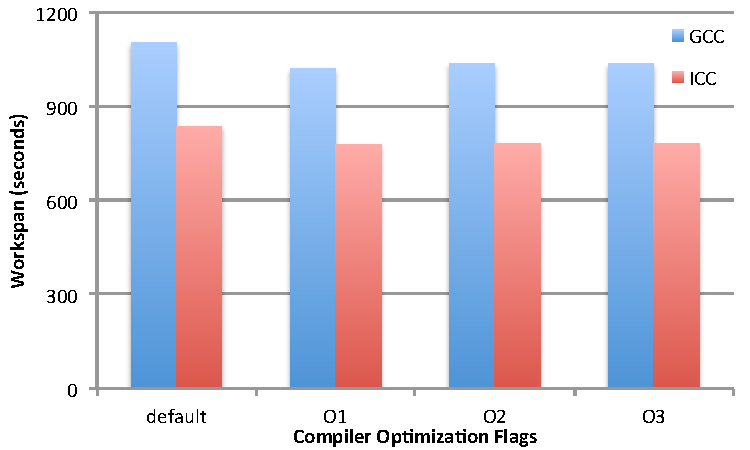
\includegraphics[width=6cm]{fig01}
\vspace{-5pt}
\caption{Compiler Optimization Results}
\vspace{-10pt}
\label{fig:compiler}
\end{figure}


Figure \ref{fig:compiler} shows the performance difference between GCC and ICC, with different compiler optimization flags. In general, ICC achieves better performance in that the makespans of the ICC test runs are 24\% shorter than the makespans of the GCC test runs. When compiler optimization flags are used, both GCC and ICC achieve additional 7\% performance gain as compared with the default version, while the difference between different compilation flags is very small.

\subsection{The Parallelization of Bottleneck Task}
\label{v1_sec:parallware}

As mBgModel is identified as the bottleneck of Montage, we present a cost-effective OpenMP-enabled parallelization strategy of mBgModel. For this purpose we use the automatic paralyzation tool available in the latest version of Parallware. The resulting OpenMP-enabled parallel mBgModel provides good performance gains at the cost of short development times. 

Below is the pseudocode of the sequential code of the task mBgModel. 

\begin{lstlisting}
struct FitInfo {
  double a, b, c;
  ...
  struct CorrInfo *plusimg;
  struct CorrInfo *minusimg;
} *fits;

struct CorrInfo {
  double a, b, c;
  double acorrection, bcorrection, ccorrection;
  ...
  struct FitInfo **neighbors;
} *corrs;

#pragma omp parallel shared(...) private(...)
{
for (t = 0; t < niterations; t++) {
  #pragma omp for schedule(static,1)
  for (i = 0; i < ncorrs; i++) {
    corrs[i].acorrection = 0;
    corrs[i].bcorrection = 0;
    corrs[i].ccorrection = 0;
    ta = 0;
    tb = 0;
    tc = 0;
    for (j = 0; j < neighbours[i]; j++) {
      ta += corrs[i].neighbors[j]->a;
      tb += corrs[i].neighbors[j]->b;
      tc += corrs[i].neighbors[j]->c;
    }
    corrs[i].acorrection = ta/2;
    corrs[i].bcorrection = tb/2;
    corrs[i].ccorrection = tc/2;
  }
  #pragma omp for
  for (k = 0; k < ncorrs; k++) {
    corrs[k].a += corrs[k].acorrection;
    corrs[k].b += corrs[k].bcorrection;
    corrs[k].c += corrs[k].ccorrection;
  }
  #pragma omp for
  for (l = 0; l < nfits; l++) {
    fits[l].a -= fits[l].plusimg->acorrection;
    fits[l].b -= fits[l].plusimg->bcorrection;
    fits[l].c -= fits[l].plusimg->ccorrection;
    fits[l].a += fits[l].minusimg->acorrection;
    fits[l].b += fits[l].minusimg->bcorrection;
    fits[l].c += fits[l].minusimg->ccorrection;
  }
}
}
\end{lstlisting}

The original source code consists of 1051 source lines of codes, according to the SLOCCount utility. The design of the data structure poses a challenge on detection of parallelism because it consists of a recursive {\em struct FitInfo}, with indirect recursion through the auxiliary {\em struct CorrInfo}. The code processes a set of astronomical images. The pixels of an astronomical image are represented as an array {\em fits[]}, and their neighbours in other images are represented in the array {\em corrs[]} and its field {\em neighbors[]}.

The algorithmic structure of the sequential mBgModel code consists of a main loop {\em for(t)} that computes {\em fits[]} and {\em corrs[]} during a fixed number of iterations {\em niterations} (line 23). In a given iteration, the values of {\em corrs[]} are updated (lines 25-46) by adding the previous value and the value of an expression that depends on {\em fits[]} through the array of {\em neighbors[]}. In addtion, the computation of {\em fits[]} is also updated (lines 48-55) with the new values of {\em corrs[]} computed at the beginning of each iteration. Thus, the main loop computes two mutually dependent variables {\em fits[]} and {\em corrs[]} that prevent parallel execution of  main loop {\em for(t)}.

In the mBgModel code finer-grained parallelism is exploited as follows. The loop {\em for(i)} can be safely executed in parallel (lines 24-40) because it computes independent values {\em corrs[i].acorrection}, {\em corrs[i].bcorrection} and {\em corrs[i].ccorrection} in each iteraion. In similar manner, {\em for(k)} and {\em for(l)} can also be executed in parallel. The only difference is that these loops compute the sum of the values (e.g., {\em corrs[k].a += corrs[k].acorrection}) accross the iterations of {\em for(t)}. As a result, these loops can be parallelized with an OpenMP directive {\em \#pragma omp parallel for}. Finally, the parallelization overhead has been minimized by creating a unique OpenMP parallel region before the main loop {\em for(t)} using {\em \#pragma omp parallel} (line 21). In order to guarantee correctness, appropriate synchronization is added so that the OpenMP threads are implicitly synchronized at the beginning of each {\em for(t)} iteration.

To examine the effect of parallelization, we first compile the whole Montage workflow with the -O2 flag. Then we compile the parallelized version of mBgModel with the -O2 flag, and use it to replace the original mBgModel binary. Then we use DEWE to run the 6.0 degree Montage workflow, and compare the results with the results obtained from the unmodified version. DEWE, similar to other workflow management systems, binds individual tasks with CPUs for the convenience of task scheduling. That is, tasks with multi-thread capability are running on a single CPU assigned to the task by the workflow management system. In this study, we modify DEWE's task handler module to remove the task to CPU binding for task mBgModel, allowing task mBgModel to using all of the CPUs available on the worker node. The computing cluster includes 4 m3.2xlarge instances, each of which has 8 vCPUs and 30 GB memory. 

Figure \ref{fig:parallel} shows the impact of parallelization on the performance of the 6.0 degree Montage workflow. For binaries compiled with GCC with -O2 compiler optimization flag, parallelizing task mBgModel can further reduce the makespan by 27\%, while the execution time for task mBgModel can be reduced by 80\%. For binaries compiled with ICC with -O2 compiler optimization flag, parallelizing task mBgModel can further reduce the makespan by 7\%, while the execution time for task mBgModel can be reduced by 68\%. After parallelizing task mBgModel, the makespan of the ICC test runs is only slightly shorter than the makespan of the GCC test runs.

\begin{figure}[t!]
\centering
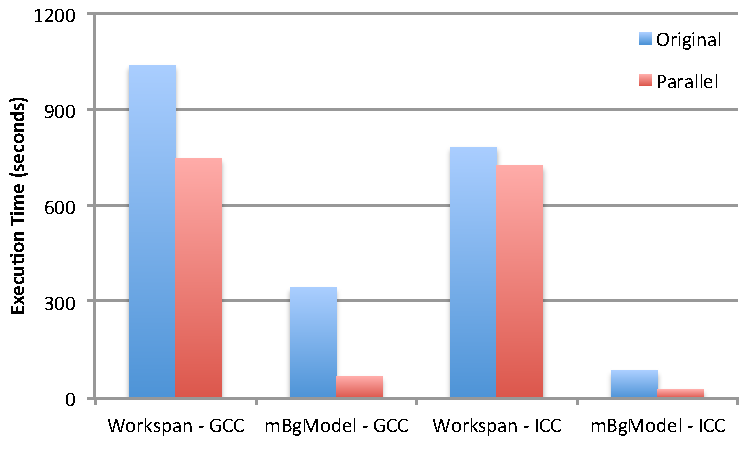
\includegraphics[height=4cm]{fig02}
\vspace{-5pt}
\caption{Impact of Parallelization on Workflow Performance}
\vspace{-10pt}
\label{fig:parallel}
\end{figure}

\subsection{Cluster Configuration}
\label{v1_sec:cluster}


Now we compare the impact of cluster configurations on the performance of Montage workflow. As shown in Table \ref{tbl:cluster}, four different clustering configurations are being tested.  Cluster M3.2X uses the m3.2xlarge instances from the M3 general purpose product family, while clusters C3.2X, C3.4X and C3.8X uses instances from the C3 compute optimized product family. All these clusters have the same number of total vCPUs. The difference lies in the size of the worker node and the number of worker nodes in the cluster.


\begin{figure}[t!]
\centering
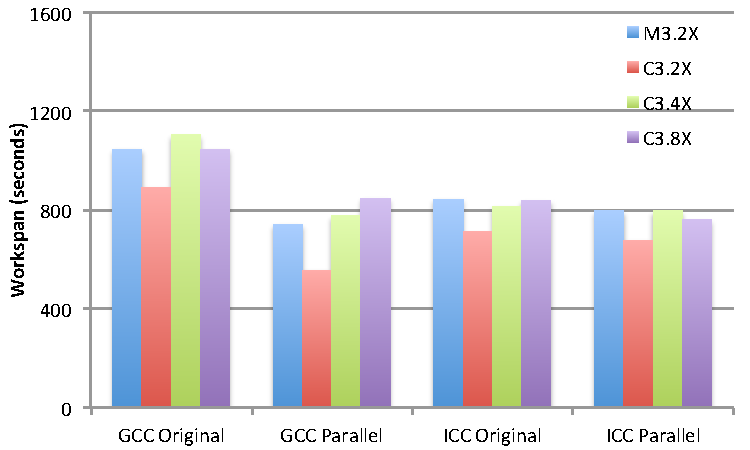
\includegraphics[width=6cm]{fig03}
\caption{Impact of Cluster Configuration - Makespan}
\label{fig:cluster}
\end{figure}

\begin{figure}[t!]
\centering
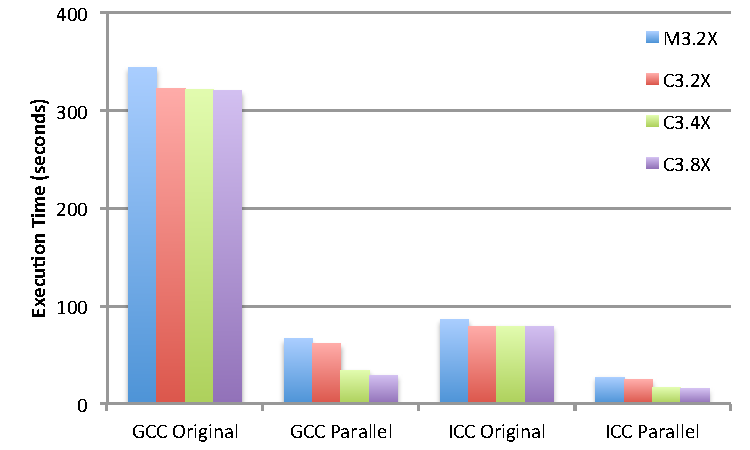
\includegraphics[width=6cm]{fig04}
\caption{Impact of Cluster Configuration - mBgModel}
\label{fig:mBgModel}
\end{figure}

\begin{figure}[t!]
\centering
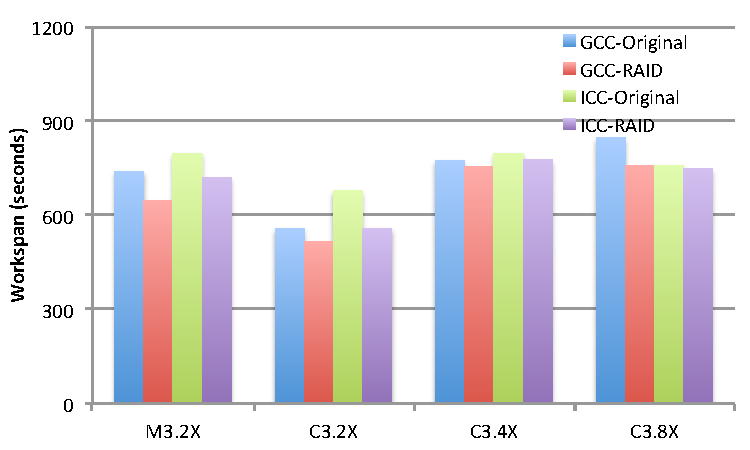
\includegraphics[width=6cm]{fig05}
\caption{Impact of RAID 0 on Makespan}
\label{fig:raid}
\end{figure}

\begin{figure}[t!]
\centering
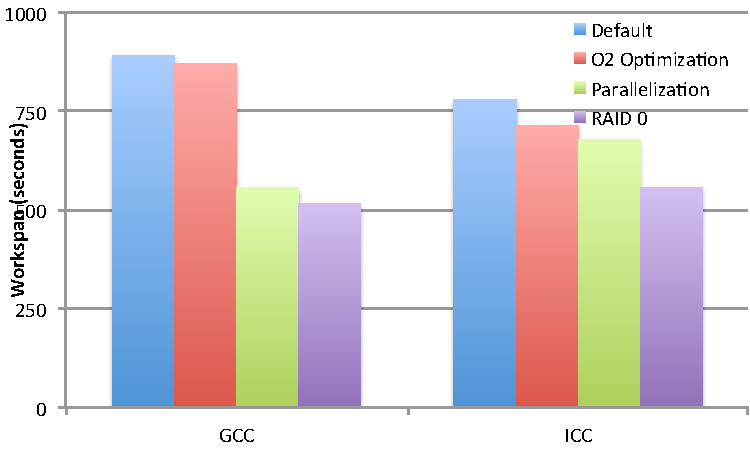
\includegraphics[width=6cm]{fig06}
\caption{Combination of Optimization Techniques}
\label{fig:combine}
\end{figure}

Figure \ref{fig:cluster} shows the impact of cluster configuration on the makespan of the 6.0 degree Montage workflow. In general, the C3.2X cluster has better performance than the other clusters. Figure \ref{fig:mBgModel} show the impact of cluster configuration on the execution time of task mBgModel. With the original version, the execution time of task mBgModel is the same for each VM type with a particular compiler. With the parallelized version, the execution time of mBgModel decreases as the number of vCPUs on the worker node increases. Such reduction in execution time is significant between C3.2X and C3.4X clusters, but is insignificant between C3.4X and C3.8X clusters. 

In order to understand the above-mentioned performance difference, we monitor the CPU and disk utilization status during the test runs. We find out that on average the CPU utilization rate is about 20 to 30 percent during the test runs, while disk utilization is about 80 to 90 percent most of the time. Considering the fact that a 6.0 degree Montage workflow produces 22,850 intermediate files during its execution, we can determine that the Montage workflow is disk I/O intensive, and disk I/O presents a bottleneck in the execution. Such a hypothesis can be verified by the resource consumption pattern as shown in Figure \ref{fig:pattern}. In order to improve disk I/O capability, we create a RAID 0 configuration using the two SSD disk available on the instances, and setup EXT3 file system on the RAID device for data storage. The binaries are compiled with the -O2 flag, and the parallelized version of mBgModel is used for the testing. As shown in Figure \ref{fig:raid}, RAID 0 further reduces the makespan for all test runs. Among all test runs, binaries compiled with GCC running on C3.2X clusters has the shortest makespan.

Apart for the demand for CPU resources, the Montage workflow is at the same time I/O intensive in that a large amount of intermediate files are created during the computation. Therefore, improving I/O performance might also be able to speed up the execution. All the VM instances being used in this research have two ephemeral SSD disks, which can be combined using redundant array of independent disks (RAID) technology for data redundancy or performance improvement. In this research, we use RAID 0  to improve I/O performance through parallelism of read and write operations across multiple disks. Figure \ref{fig:raid} shows the impact of RAID 0 on the makespan of the 6.0 degree Montage workflow. On all clusters, RAID 0 introduces various degree of performance improvement, but the performance improvement is more significant for clusters M3.2X and C3.2X.

Figure \ref{fig:combine} shows the combined effect of the above-mentioned optimization techniques. In this example, a 6.0 degree Montage workflow runs on a C3.2X cluster. For binaries compiled with GCC, the makespan can be reduced from 892 seconds to 517 seconds, representing 42\% makespan reduction. For binaries compiled with ICC, the makespan can be reduced from 779 to 558 secs, representing 28\% makespan reduction. 

\begin{table}[t!]
\caption{Different Cluster Configurations}
\label{tbl:cluster}
\centering
\begin{tabular}{|p{3.0cm}|p{3.0cm}|p{3.0cm}|p{3.0cm}|p{3.0cm}|}
\hline
Config & M3.2X & C3.2X & C3.4X& C3.8X\\ \hline
VM Type & m3.2Xlarge & c3.2Xlarge & c3.4Xlarge& c3.8Xlarge\\ \hline
VM vCPU & 8 & 8 & 16 & 32 \\ \hline
VM MEM & 30 GB & 15 GB & 30 GB & 60 GB \\ \hline
VM DISK & 2 X 80 GB & 2 X 80 GB & 2 X 160 GB & 2 X 320 GB \\ \hline
VM Price & 0.56 USD & 0.42 USD & 0.84 USD & 1.68 USD \\ \hline
Total Nodes & 4 & 4 & 2 & 1 \\ \hline
Total vCPU & 32 & 32 & 32 & 32 \\ \hline
Total Cost & 2.24 USD & 1.68 USD & 1.68 USD& 1.68 USD\\ \hline
\end{tabular}
\end{table}


\section{Summary}
\label{v1_sec:summary}

In this chapter, we use various techniques to optimize the execution of a 6.0 degree Montage workflow running on Amazon EC2. We find out that 

\begin{itemize}
	\item Workflow visualization techniques can be used to generate the resource consumption pattern, as well as identify the bottleneck of a workflow. 
	\item Compiler optimization can be used as general approach to optimize the execution of a scientific workflow. 
	\item The bottleneck identified can be further optimized with code level parallelization techniques. The results show that parallelism is the primary source of performance gain in modern computing systems.
	\item On Amazon EC2, further makespan reduction can be achieved by using different cluster configurations without impact on cost. Since Montage workflows are also I/O intensive, additional performance gain can be achieved using RAID 0, which improves I/O performance through parallelism of read/write operations.

\end{itemize}

